\documentclass{article}

\usepackage[T5]{fontenc}
\usepackage[utf8]{inputenc}
\usepackage[vietnamese]{babel}

\usepackage[
left = 1cm, 
right = 1cm,
bottom = 2cm,
top = 2cm,
]{geometry}

\usepackage{amsmath}
\usepackage{siunitx}

\usepackage{tabularx}
\usepackage{makecell}

\usepackage{graphicx}
\usepackage{float}
\usepackage{subcaption}

\usepackage{xcolor}
\definecolor{seagreen}{rgb}{0.18, 0.55, 0.34}
\usepackage{minted}
\usepackage[most]{tcolorbox}
\tcbuselibrary{minted}
% \setminted{bgcolor=gray!20}
\newtcbinputlisting{\inputcode}[3]{
  listing engine=minted,
  minted language=#1,
  minted options={
    breaklines, 
    fontsize=\small, 
    fontfamily=tt,
    linenos, 
    numbersep=3mm
  },
  listing file={#2},
  title={File: #3},
  colback=gray!10,
  colframe=seagreen,
  left=6mm,
  sharp corners,
  drop shadow,
  enhanced,
  listing only,
  breakable
}

\title{Bài tập nhóm lần 1\\
  Môn Vật lý tính toán}
\author{Nhóm 8}
\date{\today}

\usepackage{csvsimple}

\begin{document}
\maketitle

Danh sách sinh viên thực hiện
\begin{table}[H]
    \centering
    \begin{tabular}{|l|l|l|}
      \hline
      \textbf{STT} & \textbf{MSSV} & \textbf{Họ và tên} \\ \hline
      \csvreader[
      column names={index=\idx, number=\mssv, name=\fullname},
      late after line=\\ \hline
      ]{members.csv}{}{\idx & \mssv & \fullname}
    \end{tabular}
\end{table}

\tableofcontents

\section{Giải bài toán}

Các nghiệm của phương trình Schödinger trong giếng thế vuông hữu hạn có thể được tìm bằng cách giải 2 phương trình. Phương trình
\begin{equation}
    \tan z = \sqrt{\left(\frac{z_0}{z}\right)^2 - 1}
\end{equation}
cho hàm sóng dạng chẵn
\begin{equation}
    \psi(x) = 
    \begin{cases}
      B_e e^{\kappa x}, & x < -a \\
      D \cos(lx), & -a \le x \le a \\
      B_e e^{-\kappa x}, & x > a
    \end{cases}
\end{equation}
và phương trình
\begin{equation}
    -\cot z = \sqrt{\left(\frac{z_0}{z}\right)^2-1}
\end{equation}
cho hàm sóng dạng lẻ
\begin{equation}
    \psi(x) = 
    \begin{cases}
      B_o e^{\kappa x}, & x < -a \\
      C \sin(lx), & -a \le x \le a \\
      -B_o e^{-\kappa x}, & x > a
    \end{cases}
\end{equation}
trong đó, \(B_e, D, B_o, C\) là các hệ số nhận được khi áp dụng điều kiện chuẩn hóa và điều kiện biên cho hàm sóng, đối với hàm sóng dạng chẵn chúng có giá trị
\begin{equation}
    \begin{cases}
      B_e &= \sqrt{\dfrac{\kappa}{1 + \kappa a}} \cos(la) e^{\kappa a} \\
      D &= \sqrt{\dfrac{\kappa}{1 + \kappa a}}
    \end{cases}
\end{equation}
với hàm sóng dạng chẵn chúng có giá trị
\begin{equation}
    \begin{cases}
      B_o &= -\sqrt{\dfrac{\kappa}{1 + \kappa a}} \sin(la) e^{\kappa a} \\
      C &= \sqrt{\dfrac{\kappa}{1 + \kappa a}}
    \end{cases}
\end{equation}

Nhận xét bài toán, vẽ 3 hàm số sau bằng \texttt{gnuplot} (ví dụ với \(z_0 = 5\))
\begin{enumerate}
\item \(y = \tan x\)
\item \(y = -\cot x\)
\item \(y = \sqrt{\left(\dfrac{z_0}{z}\right)^2 - 1}\)
\end{enumerate}

\inputcode{gnuplot}{functions.gp}{functions.gp}
\begin{figure}[H]
    \centering
    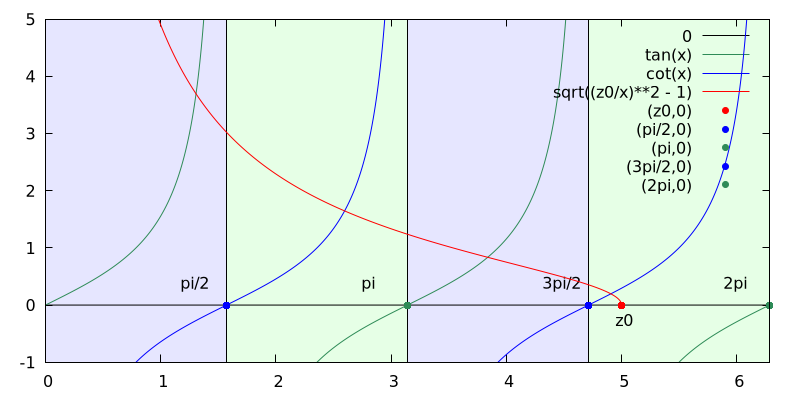
\includegraphics[width=0.75\linewidth]{images/functions.png}
\end{figure}

Nhận thấy rằng
\begin{itemize}
\item Các nghiệm cần tìm nằm trong khoảng \([0,z_0]\)
\item Nghiệm luân phiên giữa cho hàm sóng dạng chẵn và lẻ, bắt đầu với dạng chẵn
\item Các nghiệm nằm trong khoảng
    \begin{equation}
        (i - 1) \frac{\pi}{2} < x_i < i \frac{\pi}{2}
    \end{equation}
    với \(x_i\) là nghiệm thứ \(i\) (\(i = 1,2,3,\ldots\))
\item Số nghiệm đối với một giá trị \(z_0\) cho sẵn là
    \begin{equation}
        N = \left\lceil \frac{z_0}{\pi/2} \right\rceil = \left\lceil \frac{2 z_0}{\pi} \right\rceil
    \end{equation}
\end{itemize}

\section{Chương trình}

Viết thành 3 file code có nhiệm vụ khác nhau
\begin{enumerate}
\item File \texttt{methods.py} để áp dụng ba phương pháp nhằm tìm nghiệm z
\item File \texttt{plot.py} để vẽ đồ thị
\item File \texttt{main.py} chương trình chính
\end{enumerate}

\begin{table}[H]
    \begin{tabularx}{\linewidth}{|l|l|X|p{3cm}|}
      \hline
      Function & Input & Output & Phụ trách \\
      \hline
      \multicolumn{4}{|c|}{\texttt{methods.py}} \\
      \hline
      \texttt{bi} & % \\
      \texttt{(f,z0,a,b,N,eps)} & % \\
      \texttt{[c1, c2, c3, ...]} & % \\
      Linh Nhi \\

      \texttt{nr} & % \\
      \texttt{(g,z0,p0,N,eps)} & % \\
      \texttt{[p0, p1, p2, ...]} & % \\
       \\

      \texttt{sc} & % \\
      \texttt{(f,z0,p1,p2,N,eps)} & % \\
      \texttt{[p1, p2, p3, ...]} & % \\
      \\

      \hline
      \multicolumn{4}{|c|}{\texttt{plot.py}} \\
      \hline
      \texttt{wave} & % \\
      \texttt{(n,z,a,V0,coeff)} & % \\
      \texttt{x = [x1, x2, ...], y = [y1, y2, ...]} & % \\
      Thanh Trúc, \\

      \texttt{plot\_wave} & % \\
      \texttt{(n,z,a,V0,coeff,scale,e\_flag)} & % \\
      Vẽ hàm sóng thứ \(n\) ứng với nghiệm \(z\) & % \\
      Phương Trang, \\

      \texttt{plot\_all\_waves} & % \\
      \texttt{(solutions,a,V0,coeff,scale,e\_flag)} & % \\
      Vẽ hàm sóng thứ \(n\) ứng với nghiệm \(z\) & % \\
      \\
      
      \texttt{plot\_well} & % \\
      \texttt{(a,V0)} & % \\
      Vẽ giếng thế & % \\
      \\

      \hline
      \multicolumn{4}{|c|}{\texttt{plot.gp}} \\
      \hline
               & & Vẽ tương tự bằng \texttt{gnuplot} & \\

      \hline
      \multicolumn{4}{|c|}{\texttt{main.py}} \\
      \hline
      \texttt{get\_results} & % \\
      \texttt{(n,method,a,V0,coeff,N,eps)} & % \\
      \texttt{[z1, z1, z3, ...]} & % \\
      Mai Loan \\

      \texttt{output\_results} & % \\
      \texttt{(n,a,V0,filename,N,eps)} & % \\
      Xuất kết quả so sánh 3 phương pháp ra file & % \\
      Gia Bảo \\

      \texttt{get\_solutions} & % \\
      \texttt{(method,a,V0,coeff,N,eps)} & % \\
      \texttt{[z01, z01, z03, ...]} & % \\
      \\

      \texttt{plot\_single} & % \\
      \texttt{(n,solutions,a,V0,filename,scale,e\_flag,w,h)} & % \\
      Vẽ giếng thế và 1 hàm sóng & % \\
      \\

      \texttt{plot\_full} & % \\
      \texttt{(solutions,a,V0,coeff,filename,scale,e\_flag,w,h)} & % \\
      Vẽ giếng thế và các hàm sóng & % \\
      \\
      \hline
    \end{tabularx}
\end{table}
\textbf{Note:} Các bạn phụ trách có nhiệm vụ đảm bảo phần code của mình hoạt động tốt. Kiểm tra/góp ý qua lại phần code khác.

\inputcode{python}{methods.py}{methods.py}

\inputcode{python}{plot.py}{plot.py}

\inputcode{python}{main.py}{main.py}

\inputcode{gnuplot}{plot.gp}{plot.gp}

\section{Kết quả và nhận xét}

Khi chạy chương trình cho điều kiện được đề xuất: \(V_0 = \qty{83}{\mega\electronvolt}, a = \qty{2}{\femto\meter}, 2m/\hbar^2 = \qty{0.0483}{\per\mega\electronvolt\per\femto\meter\squared}\)
\begin{figure}[H]
    \centering
    \begin{subfigure}[t]{0.45\linewidth}
        \centering
        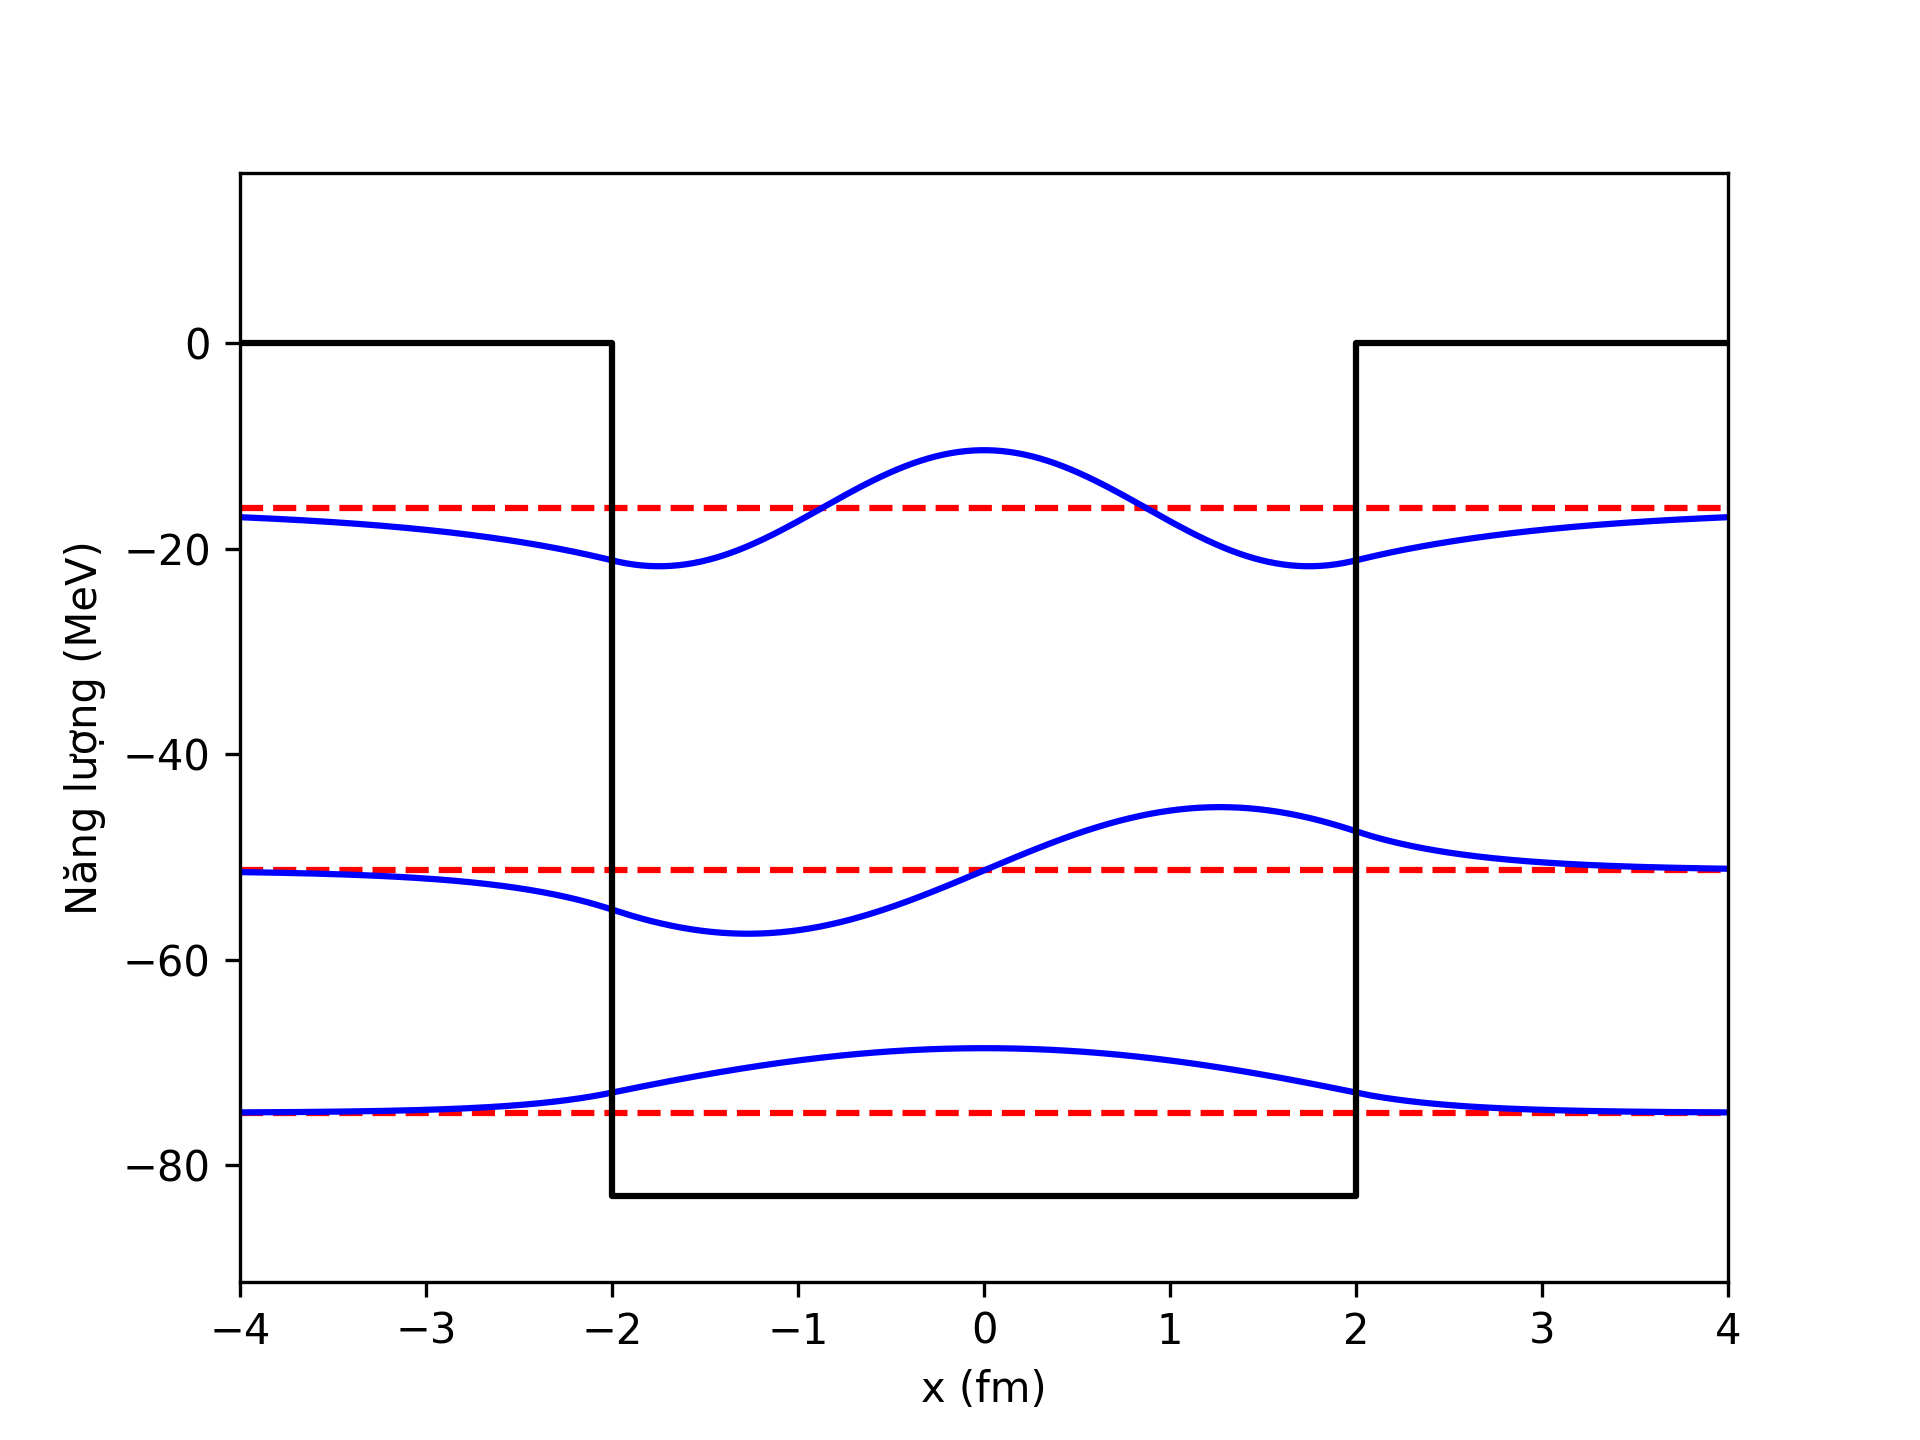
\includegraphics[width=\linewidth]{images/plot-83-2.png}
        \caption{Vẽ với \texttt{python matplotlib}}
    \end{subfigure}%
    ~ 
    \begin{subfigure}[t]{0.45\linewidth}
        \centering
        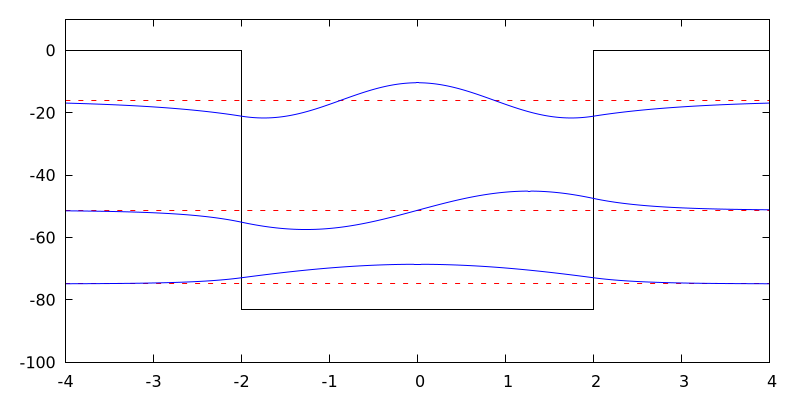
\includegraphics[width=\linewidth]{images/gnuplot-83-2.png}
        \caption{Vẽ với \texttt{gnuplot}}
    \end{subfigure}
    \caption{\(V_0 = \qty{83}{\mega\electronvolt}, a = \qty{2}{\femto\meter}\)}
\end{figure}

\begin{figure}[H]
    \centering
    \centering
    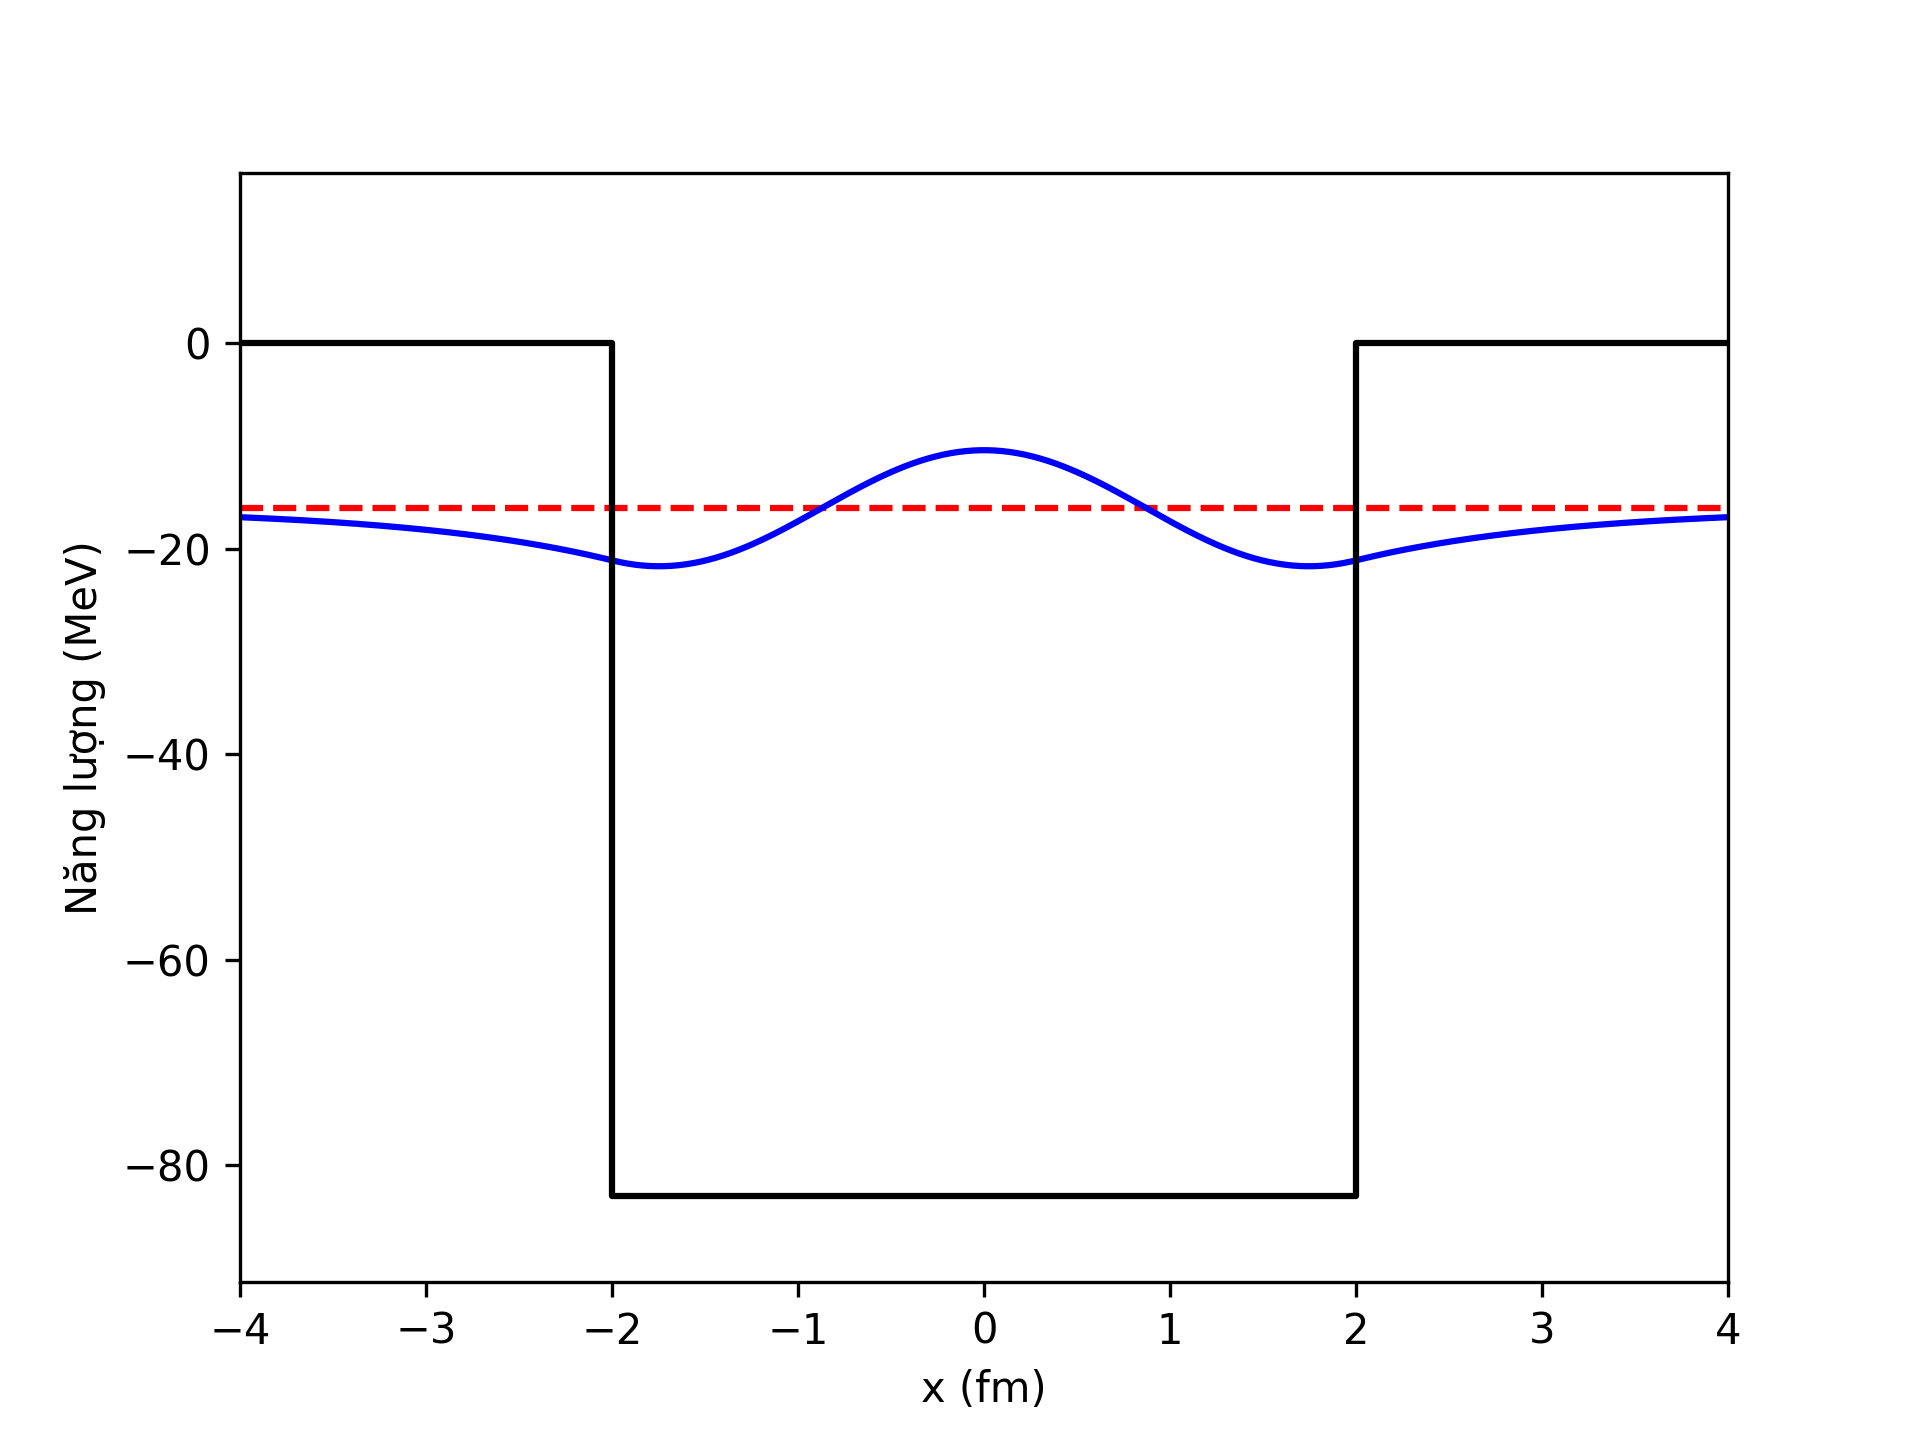
\includegraphics[width=0.5\linewidth]{images/plot-83-2-single.png}
    \caption{Hàm sóng ở mức năng lượng thứ 3}
\end{figure}

Kết quả chạy từng bước giữa 3 phương pháp được thể hiện qua dữ liệu lúc tính hàm sóng thứ 3:
\inputcode{text}{data/results-table.txt}{results-table.txt}
qua đó, thu được kết quả tương tự như các bài tập đã làm, tốc độ hội tụ của các phương pháp theo thứ tự giảm dần là: Newton-Raphson, secant, bisection.

Kết quả khi chạy chương trình cho các trường hợp giếng thế hẹp, nông và giếng thế rộng, sâu thể hiện rõ rằng giếng càng lớn thì hệ càng tiến về dạng giếng thế vuông vô hạn, giếng càng nhỏ thì hệ tiến về dạng hạt tự do. Hình vẽ hàm sóng ví dụ cho các trường hợp trên như sau:

\begin{figure}[H]
    \centering
    \begin{subfigure}[t]{0.45\linewidth}
        \centering
        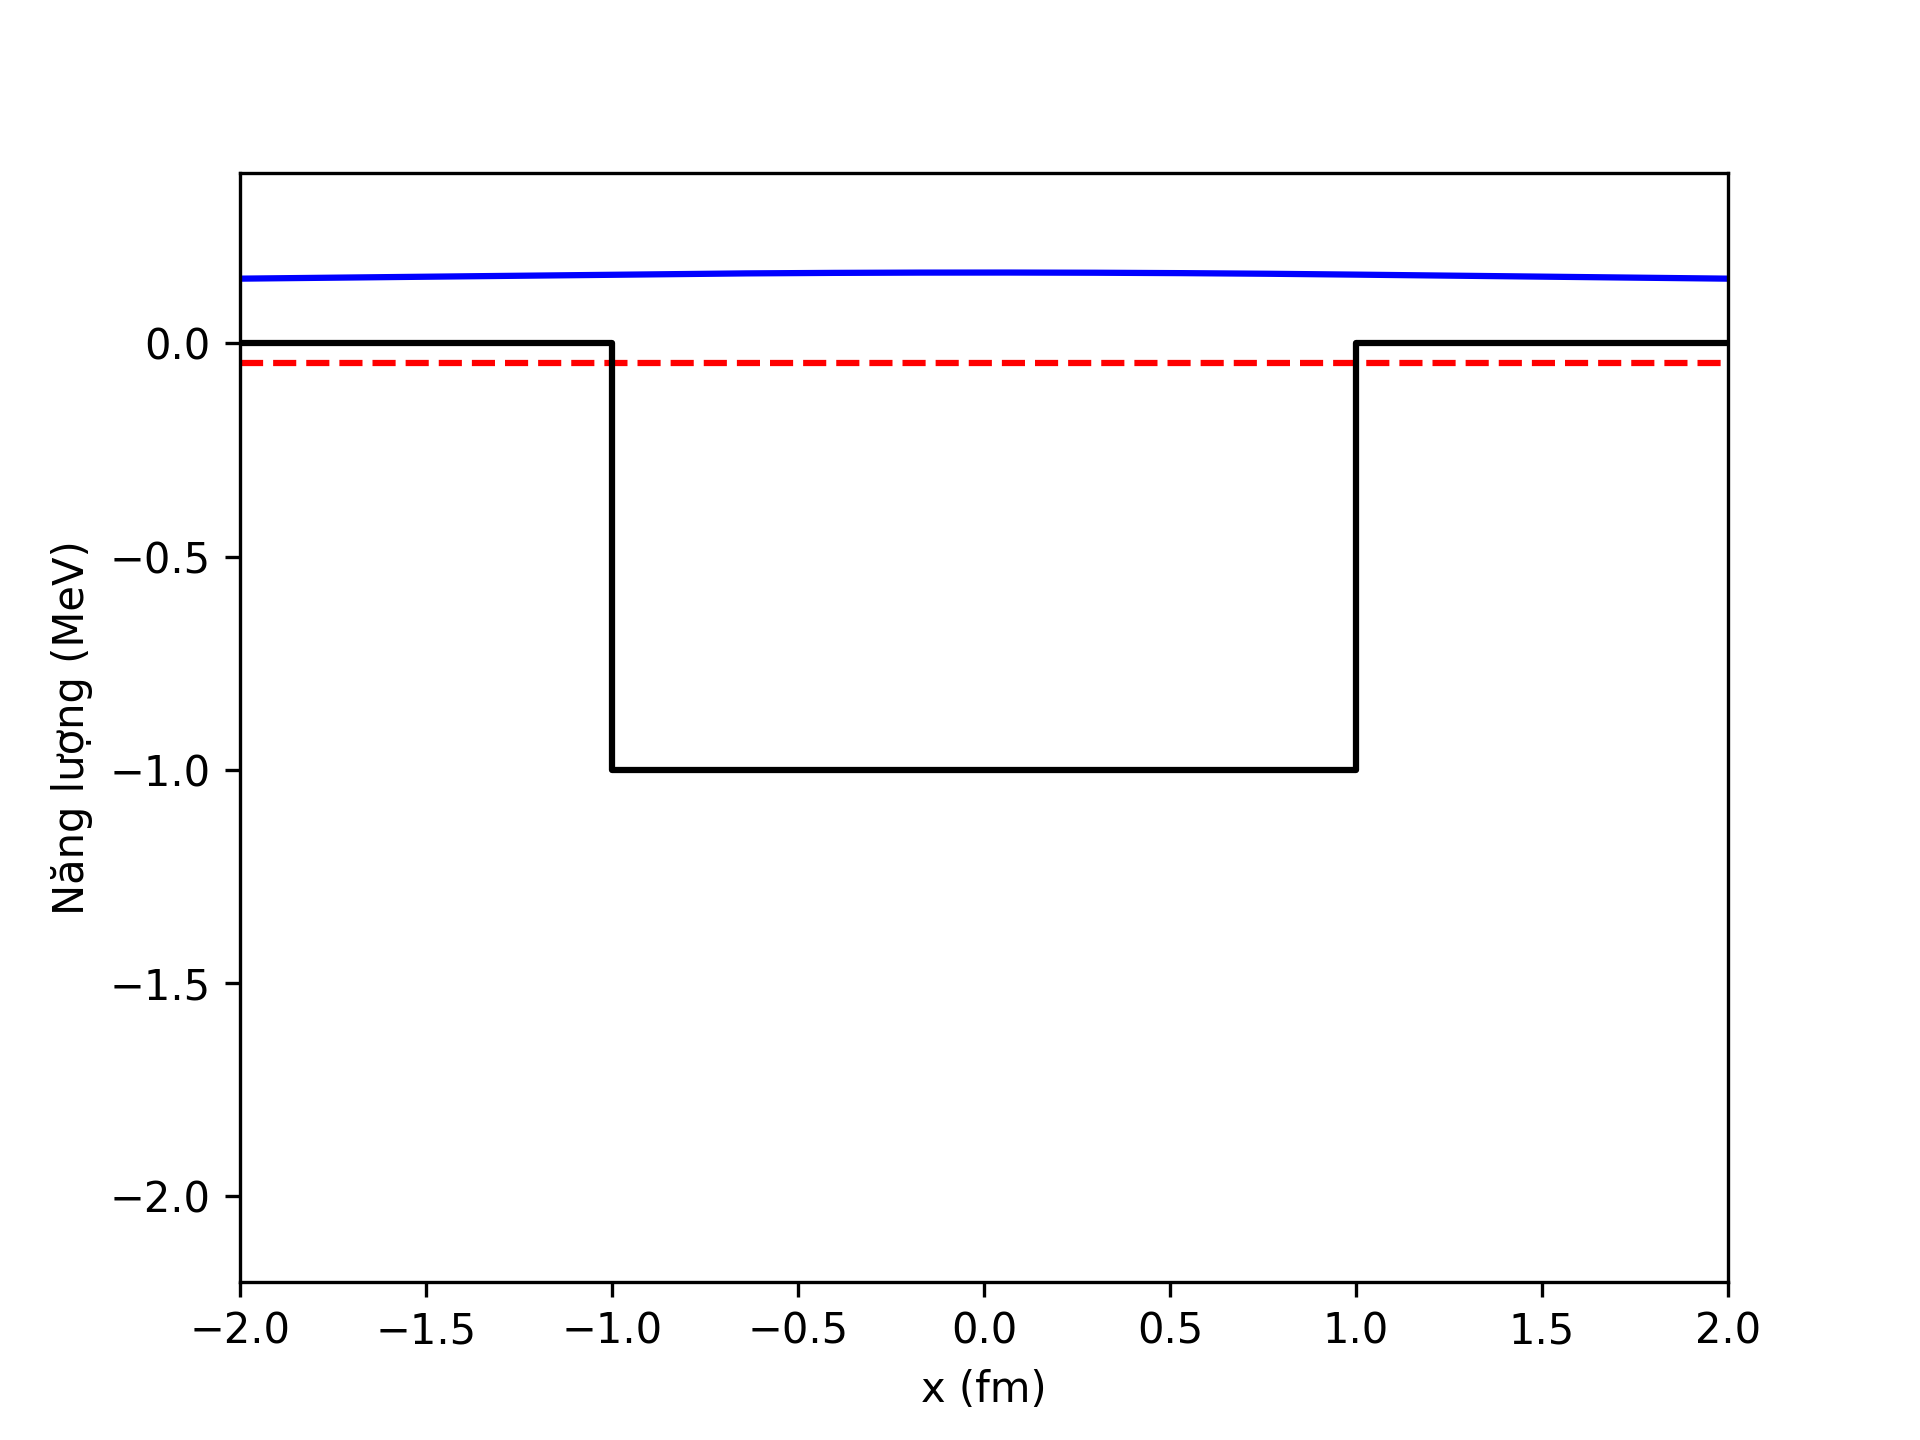
\includegraphics[width=\linewidth]{images/plot-1-1.png}
        \caption{\(V_0 = \qty{1}{\mega\electronvolt}, a = \qty{1}{\femto\meter}\)}
    \end{subfigure}%
    ~ 
    \begin{subfigure}[t]{0.45\linewidth}
        \centering
        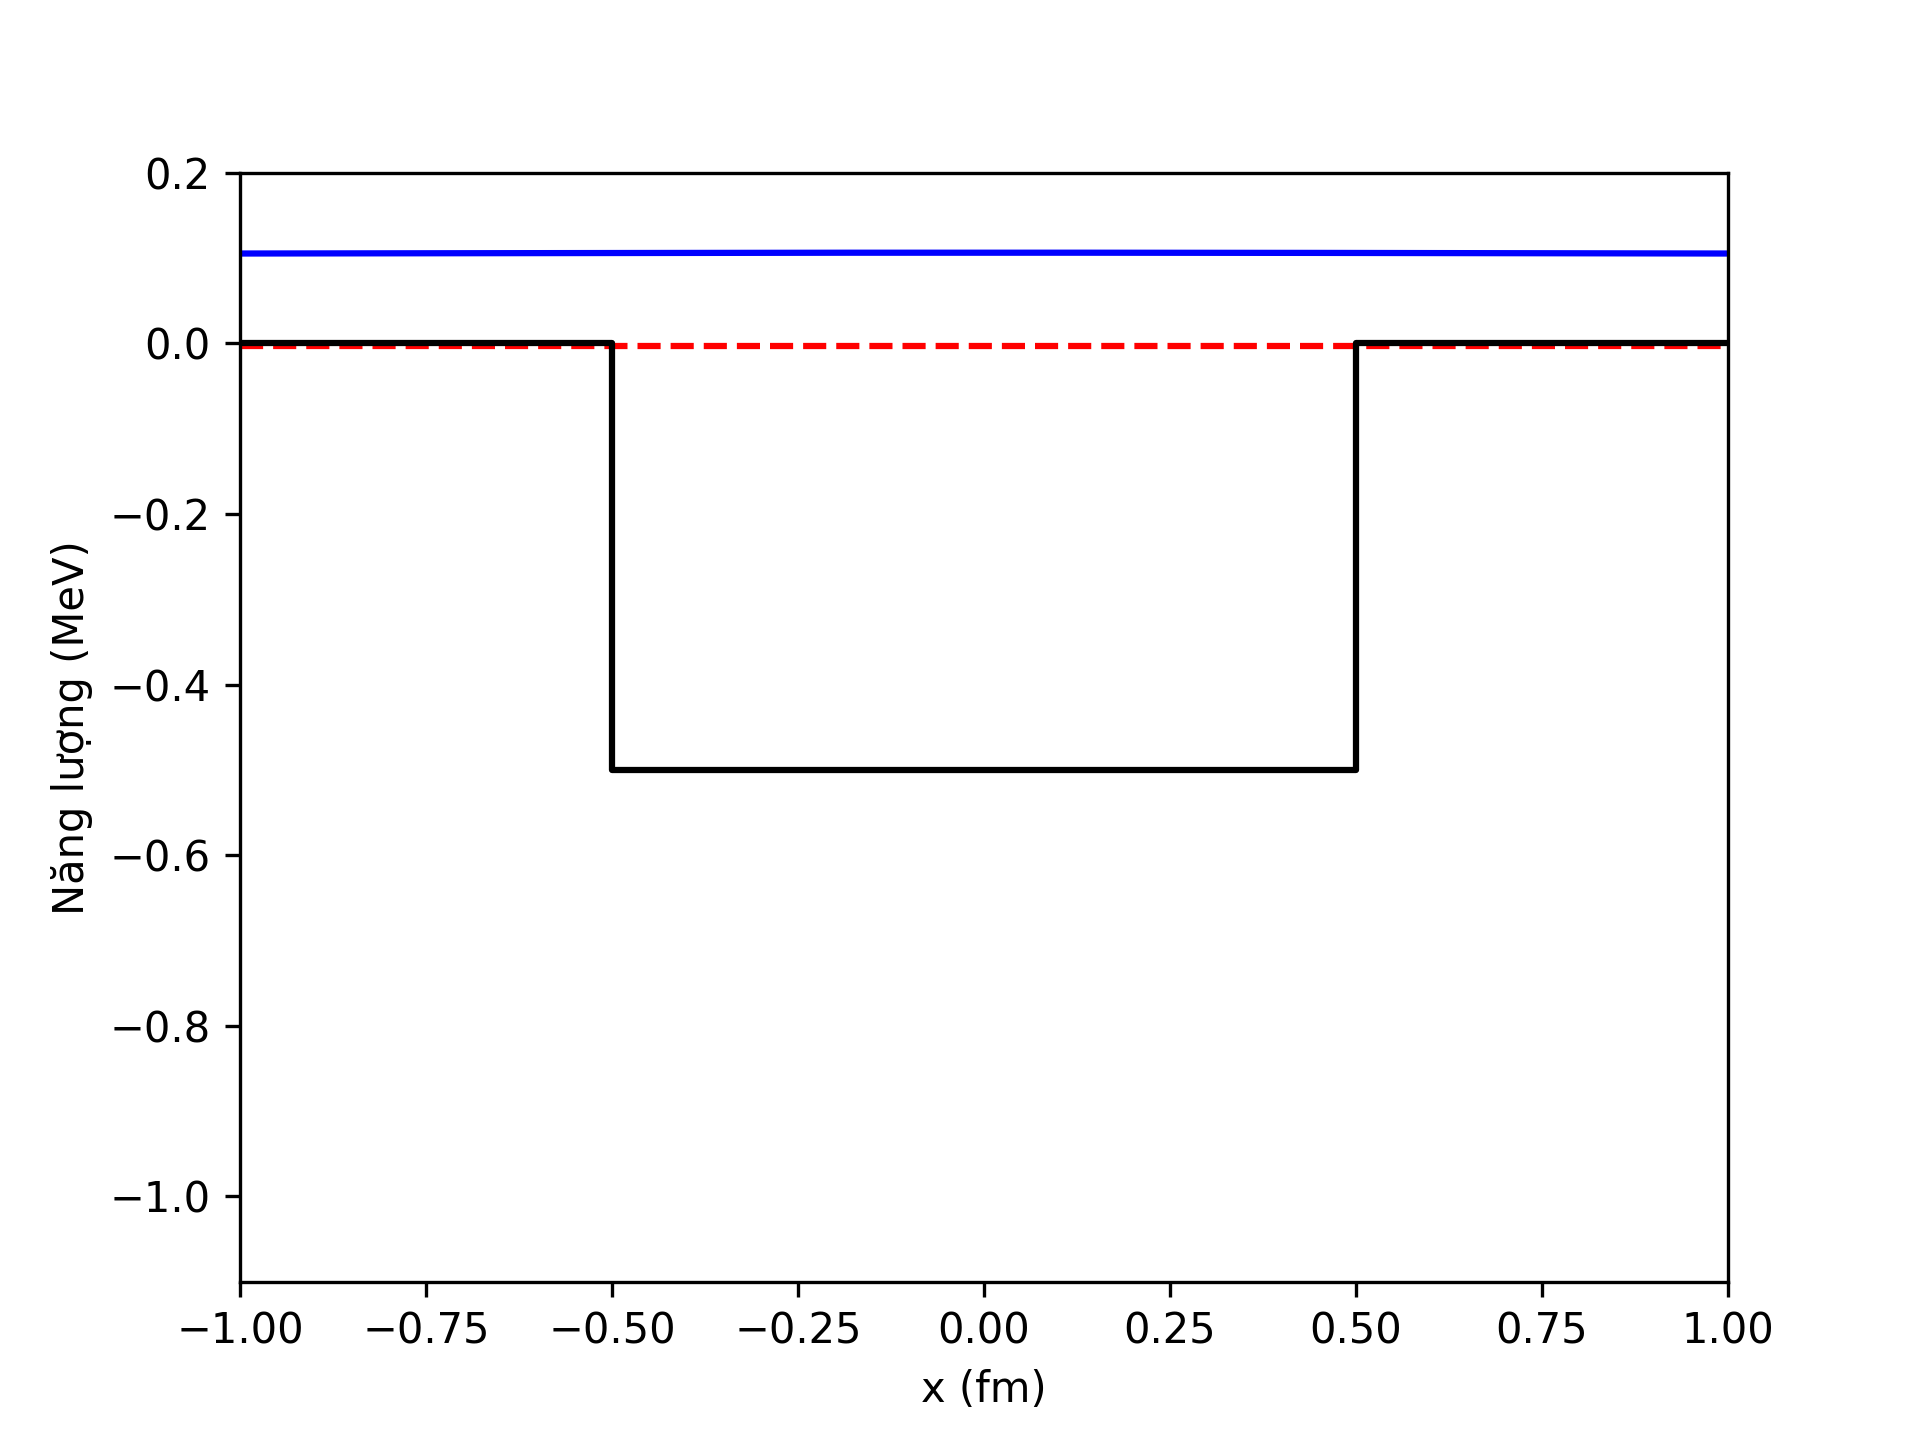
\includegraphics[width=\linewidth]{images/plot-05-05.png}
        \caption{\(V_0 = \qty{0.5}{\mega\electronvolt}, a = \qty{0.5}{\femto\meter}\)}
    \end{subfigure}
    \caption{Giếng thế hẹp và nông}
\end{figure}

\begin{figure}[H]
    \centering
    \begin{subfigure}[t]{0.45\linewidth}
        \centering
        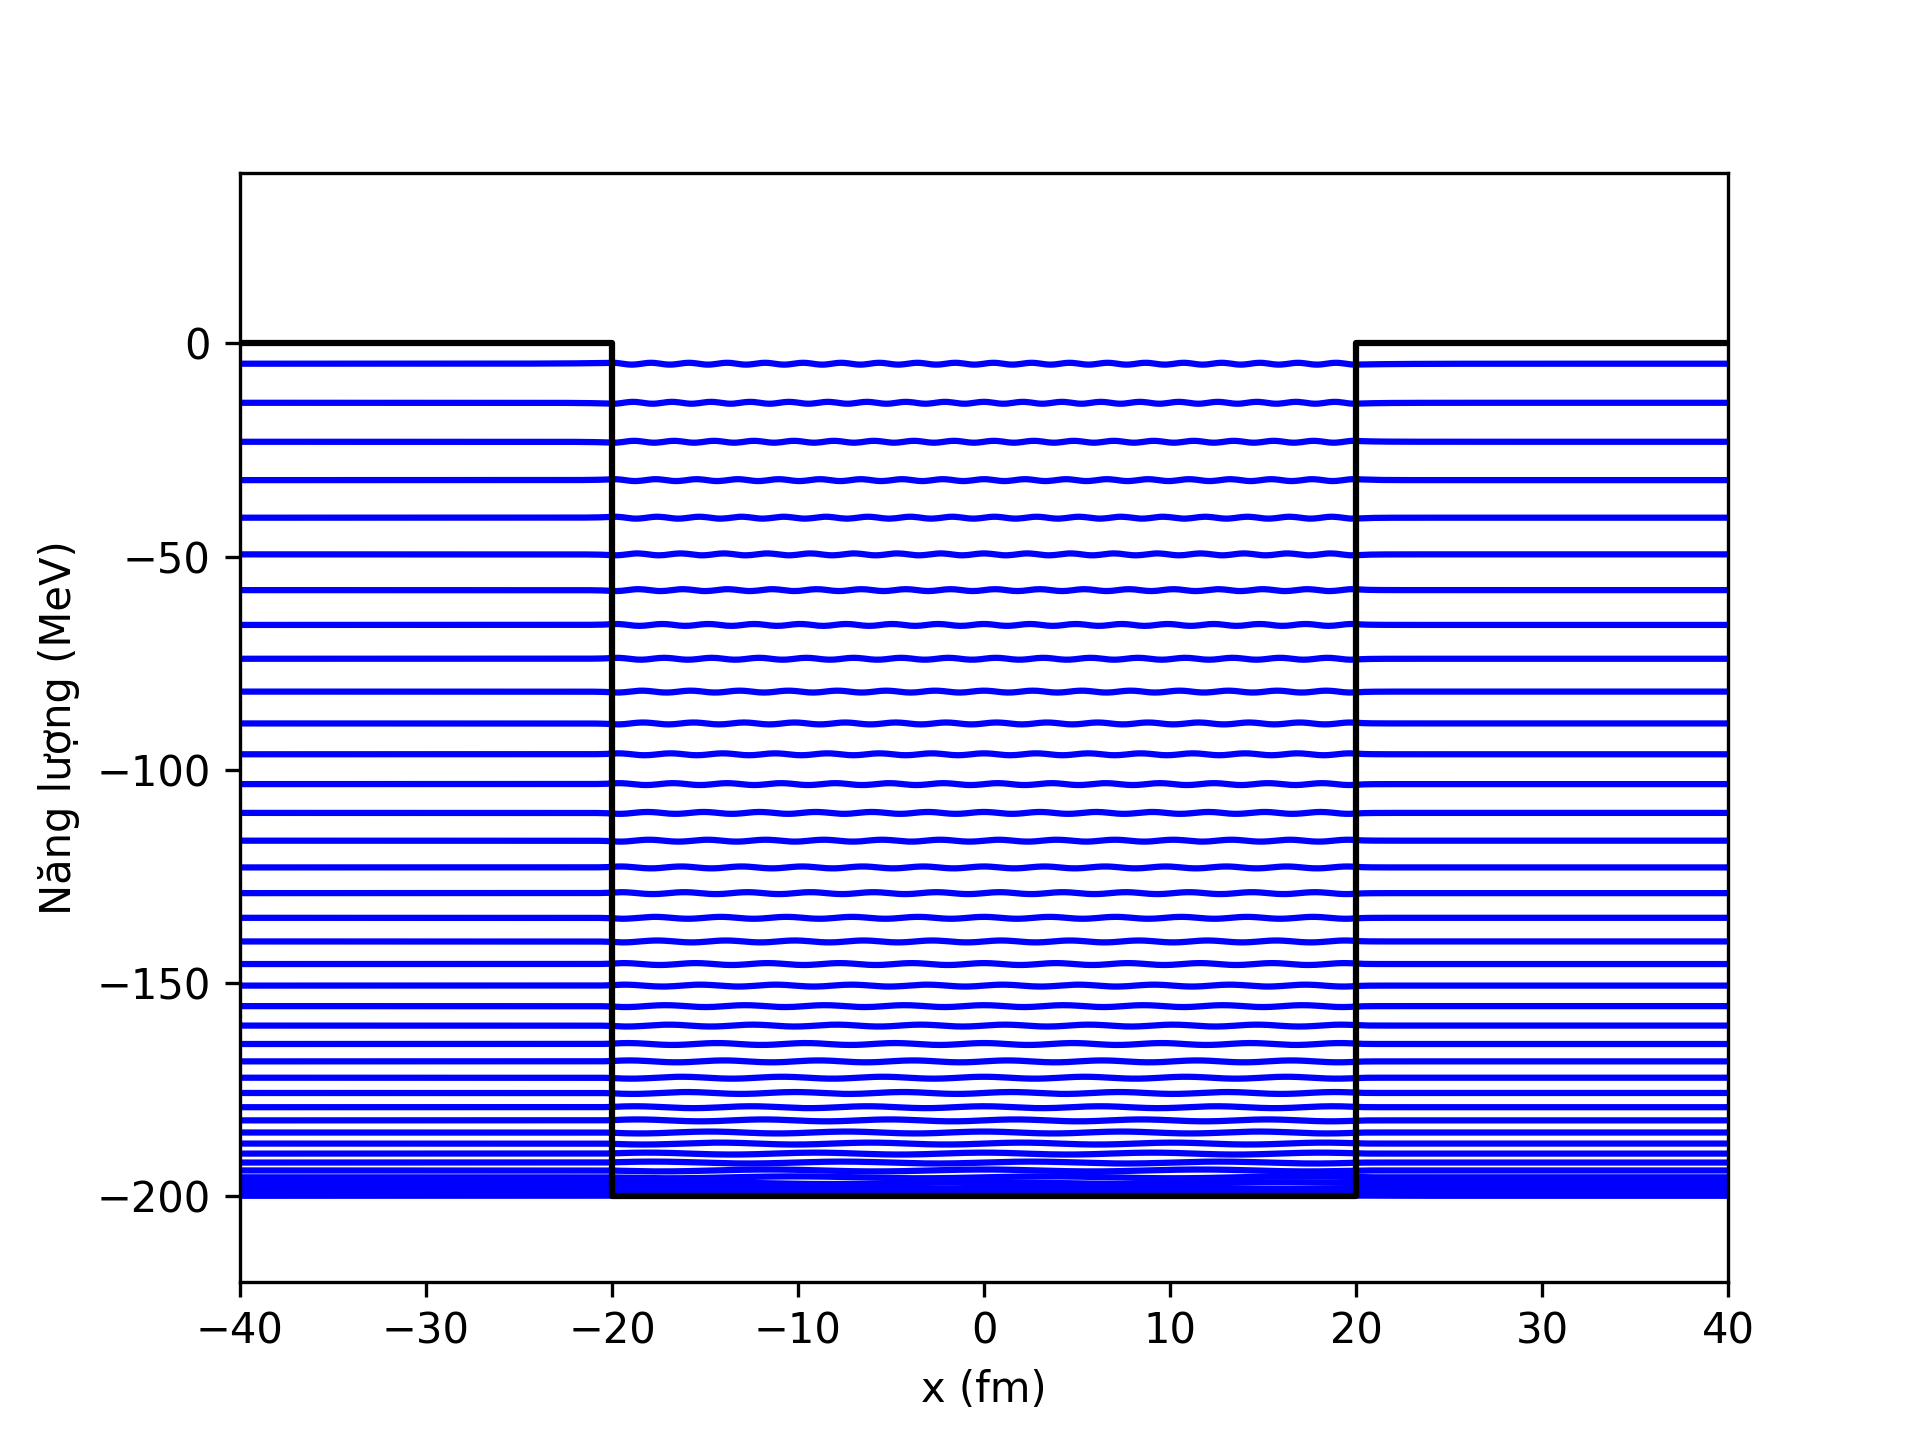
\includegraphics[width=\linewidth]{images/plot-200-20.png}
        \caption{\(V_0 = \qty{200}{\mega\electronvolt}, a = \qty{20}{\femto\meter}\)}
    \end{subfigure}%
    ~ 
    \begin{subfigure}[t]{0.45\linewidth}
        \centering
        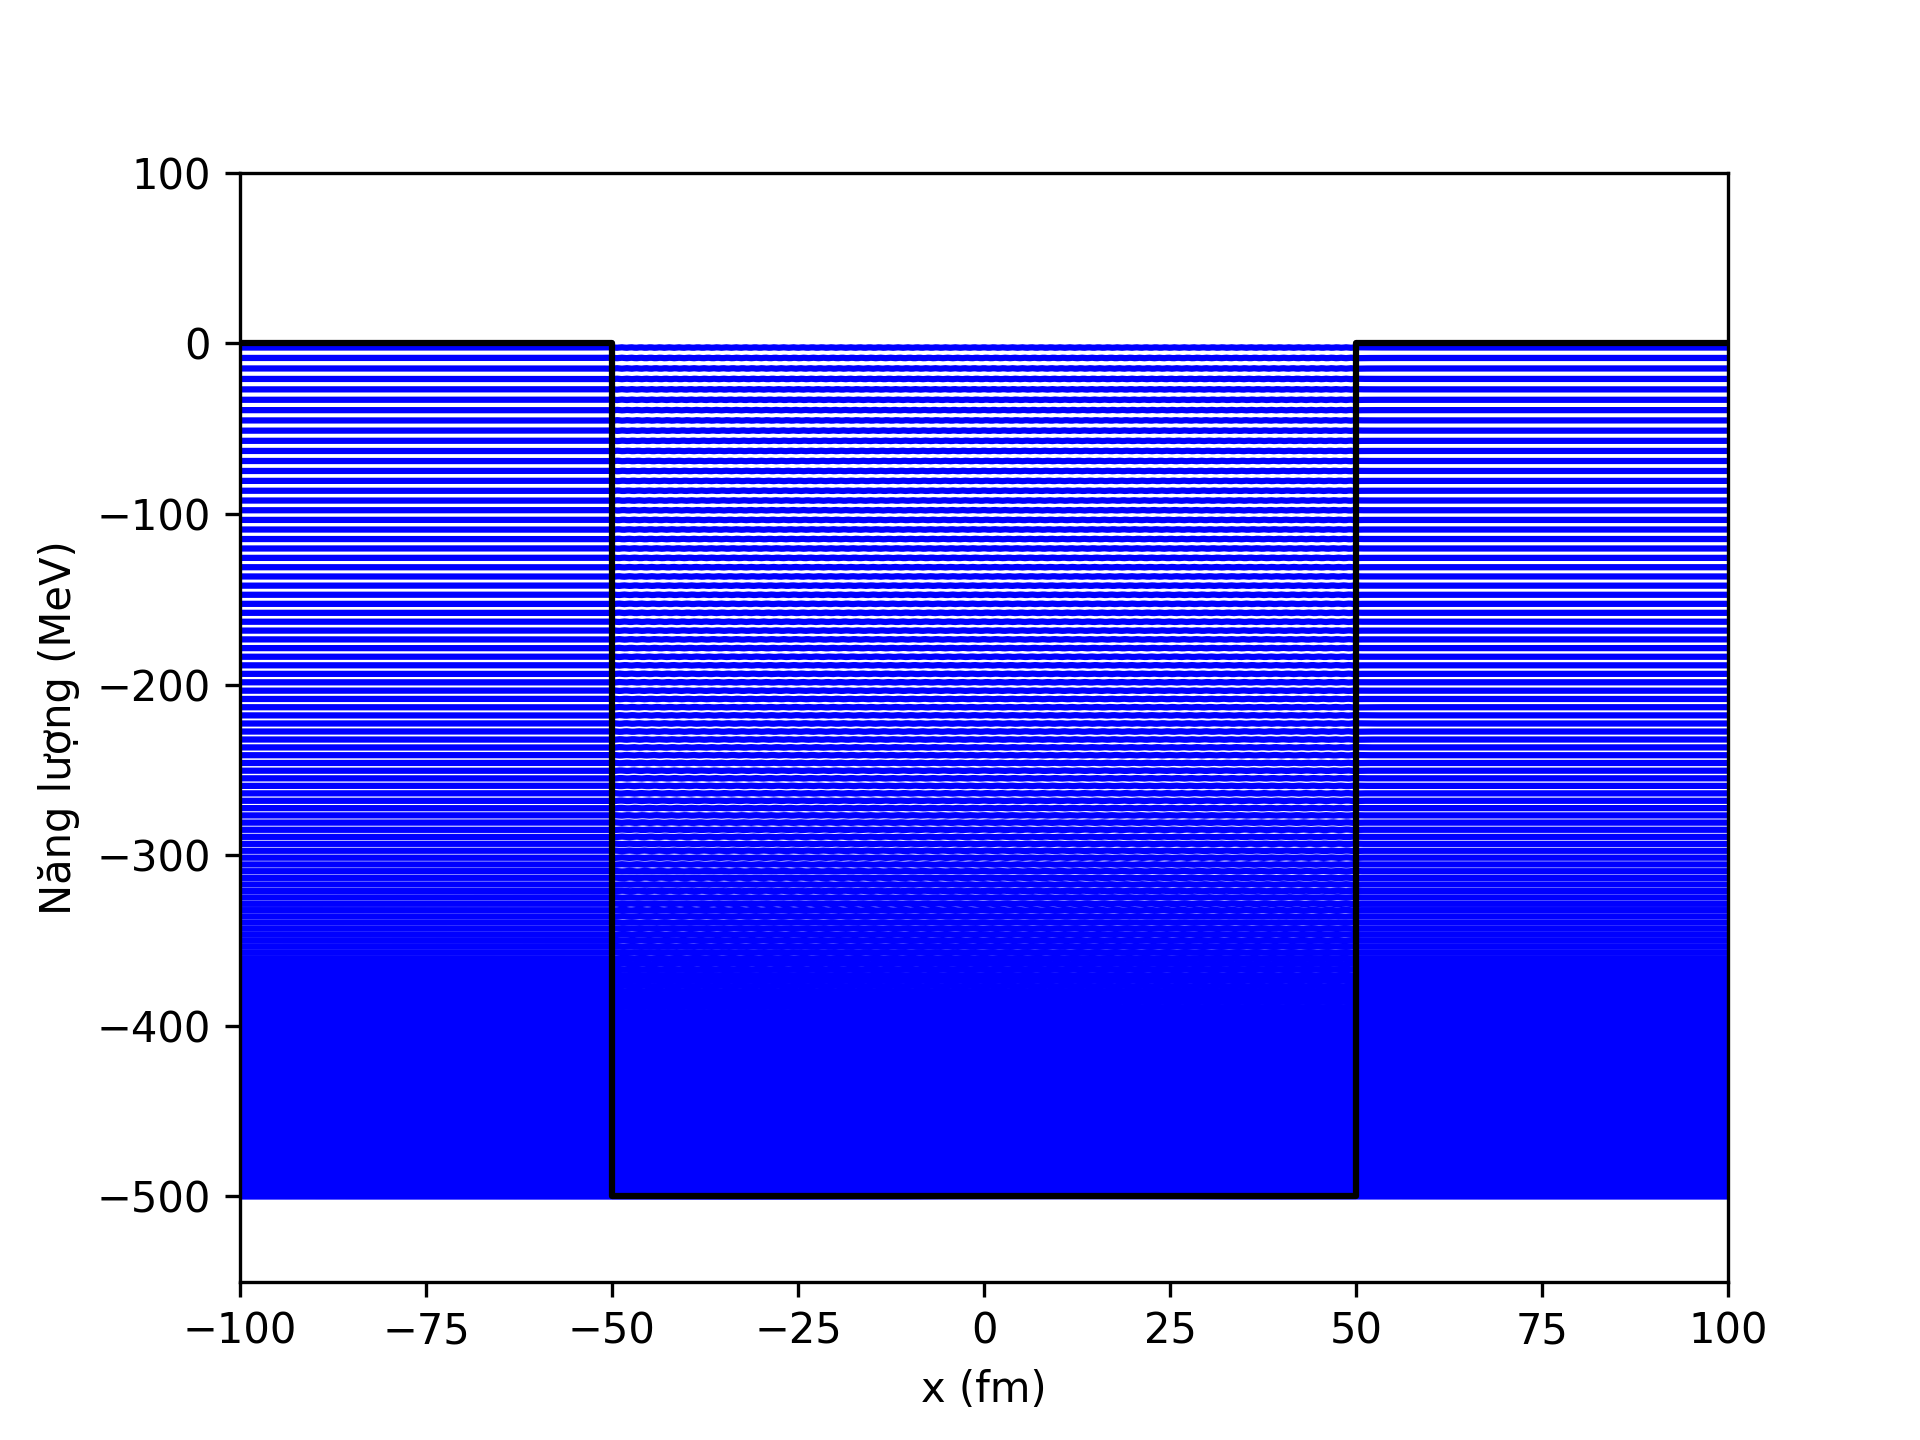
\includegraphics[width=\linewidth]{images/plot-500-50.png}
        \caption{\(V_0 = \qty{500}{\mega\electronvolt}, a = \qty{50}{\femto\meter}\)}
    \end{subfigure}
    \caption{Giếng thế rộng và sâu}
\end{figure}

\end{document}
